\documentclass[presentation]{subfiles}

\begin{document}
\begin{frame}{Introduction}
  You've learned about using Mechanical Turk through the website
  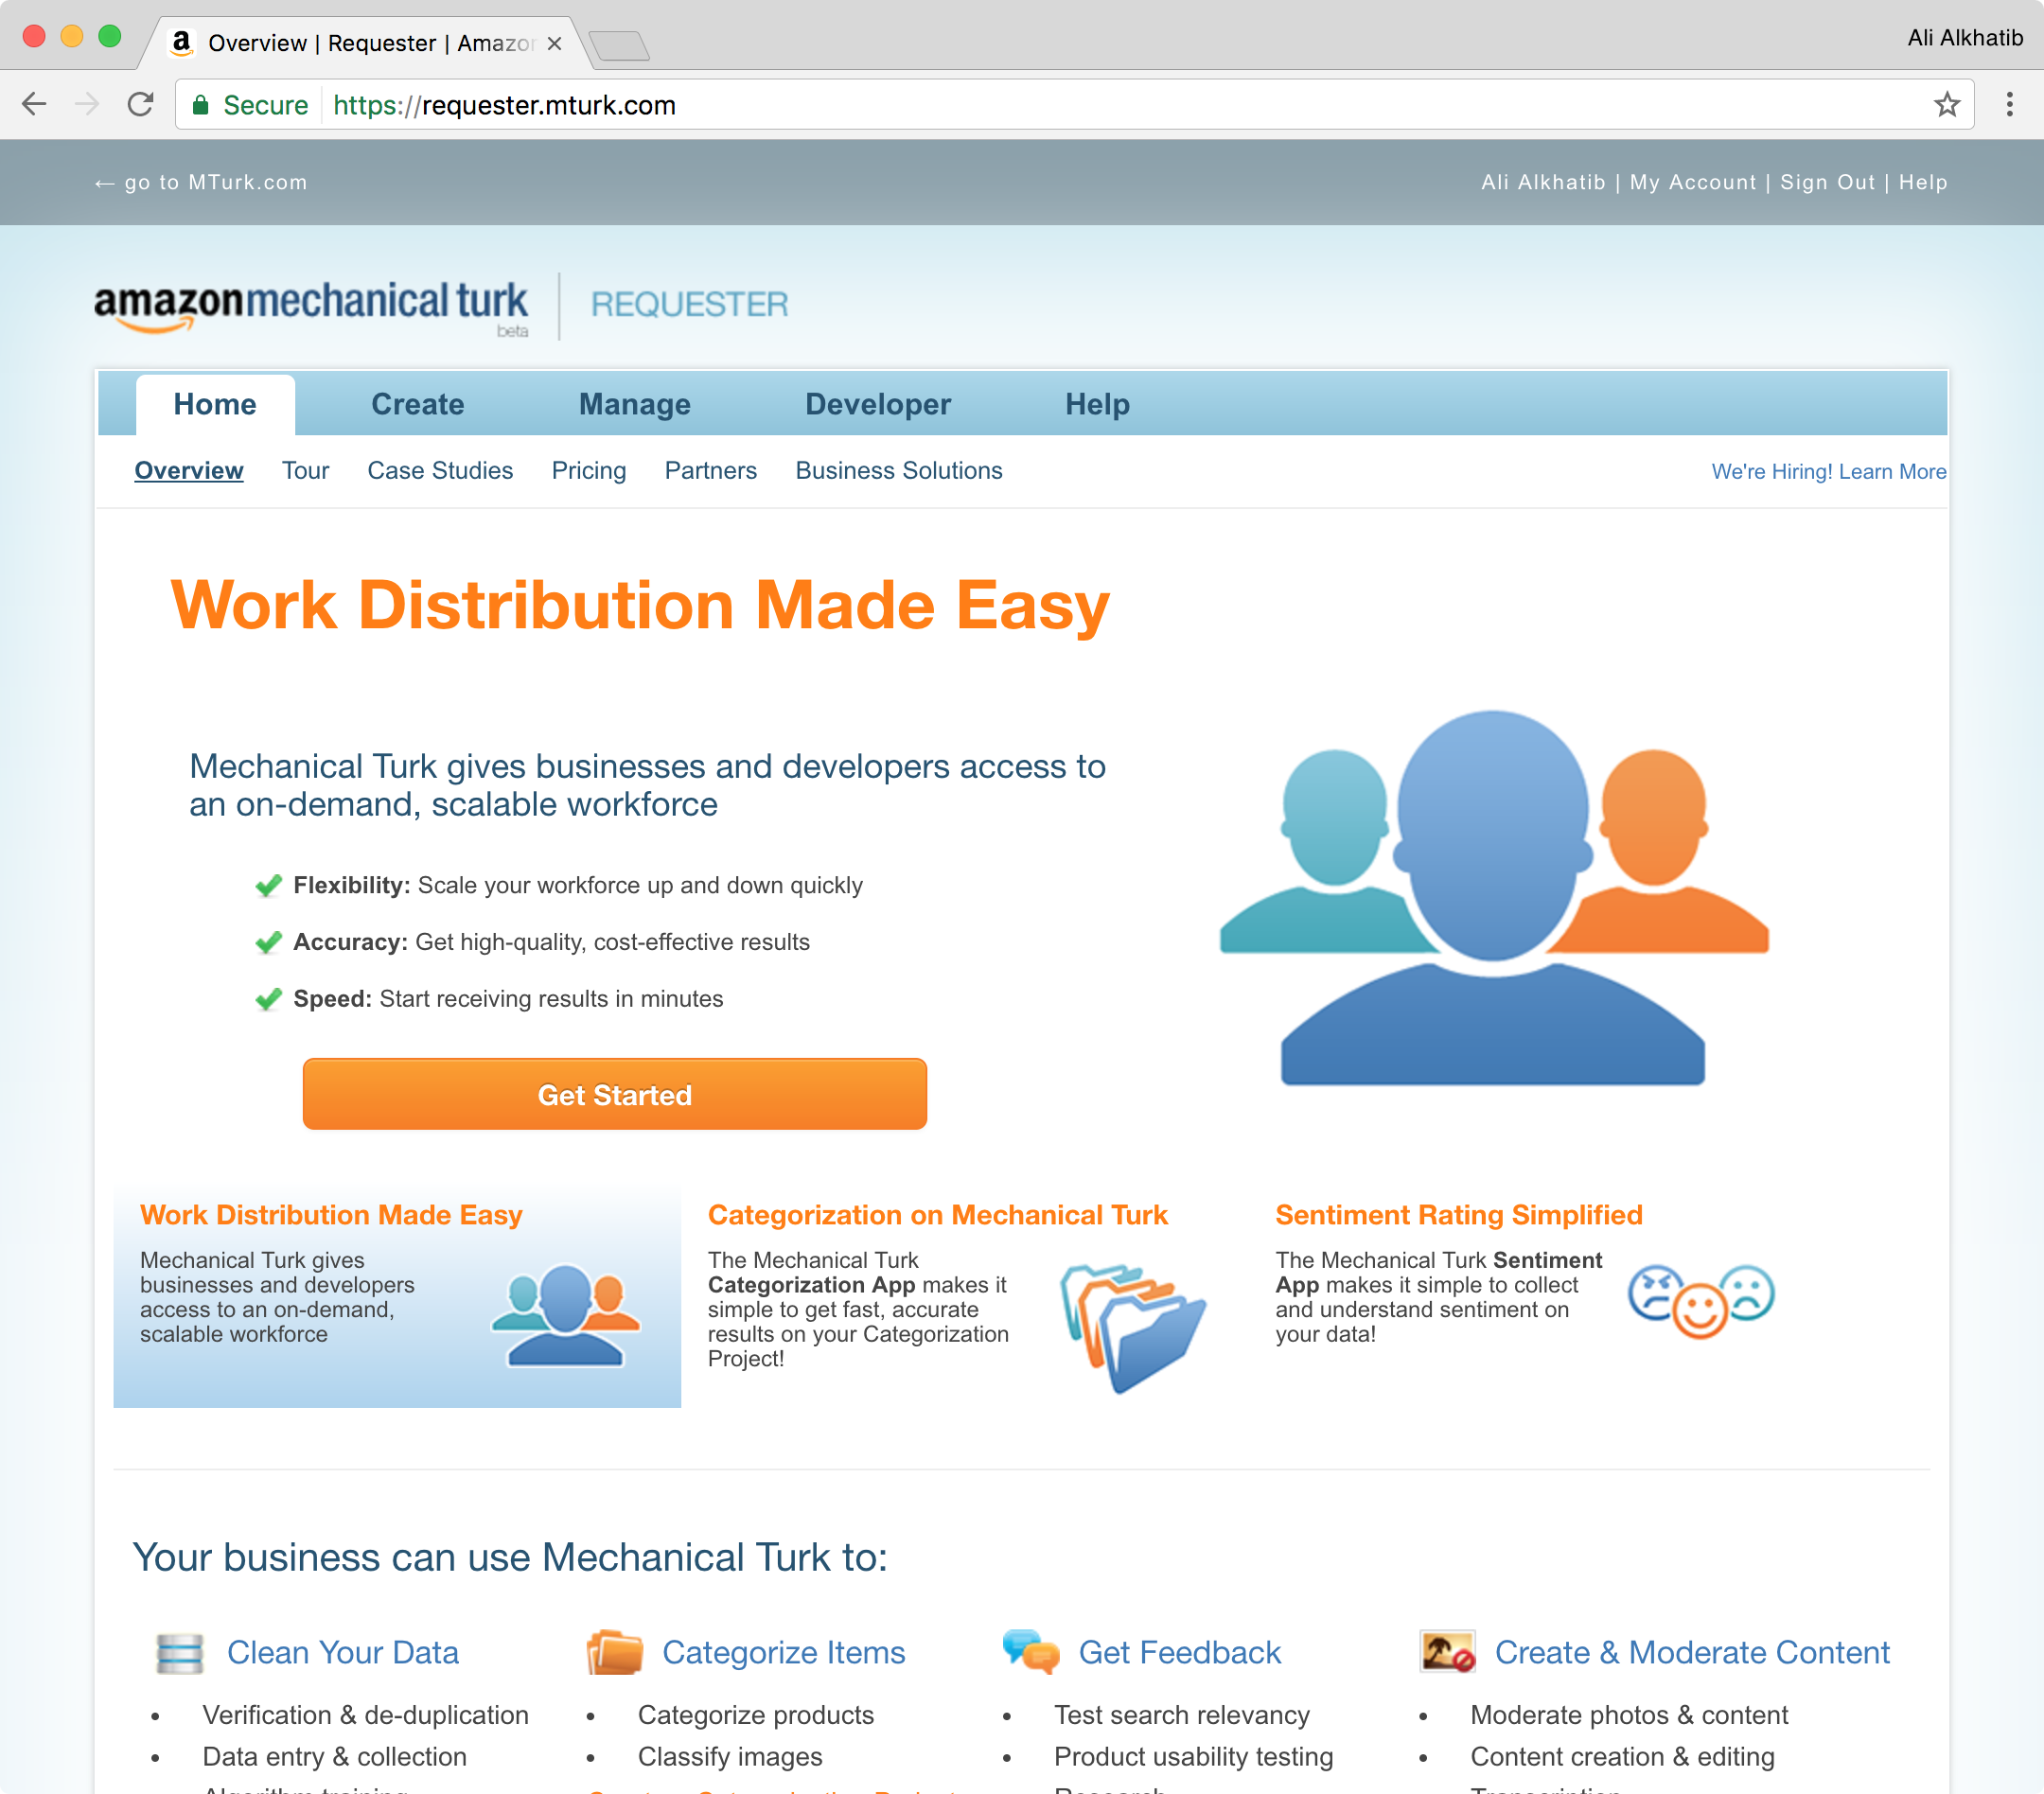
\includegraphics[width=\textwidth]{figures/amt_gui.png}
\end{frame}

\begin{frame}{Introduction}
  I'm going to give you a \emph{brief} overview of how you can do some of the same things
  with the Amazon Web Services (AWS) Software Development Kit (SDK)
\end{frame}

\begin{frame}{SDK Options}
\begin{columns}[T]
\begin{column}{0.45\textwidth}
    \begin{itemize}
      \item Java
      \item .NET
      \item Node.js
      \item Python
      \item Ruby
      \item (some more stuff here)
    \end{itemize}
\end{column}
\begin{column}{0.55\textwidth}
\begin{columns}
\begin{column}{0.5\textwidth}
\begin{itemize}
  \item[] 
\includegraphics[height=40pt]{figures/java.png}
  \item[] 
\includegraphics[height=40pt]{figures/nodejs.png}
  \item[] 
\includegraphics[height=40pt]{figures/ruby.png}
\end{itemize}
\end{column}
\begin{column}{0.5\textwidth}
\begin{itemize}
  \item[] 
\includegraphics[height=40pt]{figures/python.png}
  \item[] 
\includegraphics[height=40pt]{figures/net.png}
\end{itemize}
\end{column}
\end{columns}
\end{column}
\end{columns}
\end{frame}

\begin{frame}{Live code alert}
    I'll be using Python 3.6.1 (and, importantly, the \texttt{boto3} package, which Amazon maintains), but
    the basics are roughly the same, and all of the documentation is available at
    \url{https://aws.amazon.com/tools}

    And you can find all of this stuff at \url{https://github.com/alialkhatib/amt_tutorial}

    (if you can't find what you should be finding, please email me! $\rightarrow$
    \url{ali.alkhatib@cs.stanford.edu})
\end{frame}


\end{document}